\section{Cayley graphs}
\label{cayley}
We have seen in \cref{delooping-hit} that a delooping of~$G$ can be obtained by
further homotopy quotienting a delooping of~$\freegroup X$. The kernel of the
map $\freegroup\gamma:\freegroup X\to G$ measures the defect of~$\freegroup X$
from being~$G$, which corresponds to the relations of the group. We show here
that, under the delooping operation, those relations are precisely encoded by
the Cayley graph~\cite{cayley1878desiderata,lyndon1977combinatorial}, a
classical and useful construction in group theory which can be associated to any
generated group.

The \emph{Cayley graph} of~$G$, with respect to the generating set~$X$, is the directed graph whose
vertices are the elements of~$G$, and such that for every vertex $g:G$ and generator $x:X$,
we have an edge $g\to gx$. In homotopy type theory, it is thus natural to
represent it as the higher inductive type $\Cayley XG$ defined as
\[
  \begin{array}{l@{\ :\ }l}
    \cvertex&G\to\Cayley XG\\
    \cedge&(g:G)(x:X)\to\cvertex g=\cvertex(gx)
  \end{array}
\]
For instance, the Cayley graphs associated to $\Z_5$ (with $2$ as generator)
and $D_5$ (with $r$ and $s$ as generators) are respectively
\[
  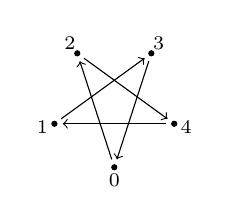
\begin{tikzpicture}[baseline=(b.base),scale=.8,every edge/.append style = {shorten <=3,shorten >=3}]
    \coordinate (b) at (0,0);
    \foreach \i in {0,...,4} {
      \filldraw ({(\i+3/4)*360/5}:1) circle (.04);
      \draw ({((-\i+3)+3/4)*360/5}:1.2) node {$\scriptstyle\i$};
      \draw[shorten <=2,shorten >=2] ({(\i+3/4)*360/5}:1) edge[<-] ({(\i+2+3/4)*360/5}:1);
    }
    % \draw (0,-1.6) node {$m=5$};
  \end{tikzpicture}
  \qquad\qquad\qquad\qquad
  \begin{tikzpicture}[baseline=(b.base),scale=.8,every edge/.append style = {shorten <=2,shorten >=2}]
    \coordinate (b) at (0,0);
    \foreach \i in {0,...,4} {
      \filldraw ({(\i+3/4)*360/5}:1) circle (.04);
      \filldraw ({(\i+3/4)*360/5}:.4) circle (.04);
      \draw ({(\i+3/4)*360/5}:1) edge[<-,inner sep=0.2ex,"$\scriptstyle r$"'] ({(\i+1+3/4)*360/5}:1);
      \draw ({(\i+3/4)*360/5}:.4) edge[->,inner sep=0.2ex,"$\scriptstyle r$"'] ({(\i+1+3/4)*360/5}:.4);
      \draw ({(\i+3/4)*360/5}:1) edge[->,bend right,gray,inner sep=0.1ex,"$\scriptstyle s$"'] ({(\i+3/4)*360/5}:.4);
      \draw ({(\i+3/4)*360/5}:.4) edge[->,bend right,gray,inner sep=0.1ex,"$\scriptstyle s$"'] ({(\i+3/4)*360/5}:1);
    }
  \end{tikzpicture}
\]
Our main result in this section is that this type satisfies the following
property. We recall that the delooping operation is functorial, see
\cref{delooping-functorial} and~\cite{warn2023eilenberg}: in particular, we can
deloop morphisms. We also recall that the \emph{kernel} of a map $f:A\to B$ with $B$ pointed is its fiber at the distinguished element $\pt{}$ of~$B$.

\begin{theorem}[\agda{Cayley}{Cayley-ker}]
  \label{flattening-cayley}
  The type $\Cayley XG$ is the kernel of the function $\B\freegroup \gamma:\B\freegroup X\to\B G$ induced by~$\gamma$, \ie we have
  \[
    \Cayley XG
    \qeq
    \Sigma(x:\B X^*).(\pt{}=\B\freegroup\gamma(x))
    \text.
  \]
\end{theorem}
\begin{proof}
  We define the type family $P:\B\freegroup X\to\U$ by
  $P(x)=(\pt{}=\B\freegroup \gamma(x))$. Remember that $\B\freegroup X$ admits a
  description as a coequalizer, see \cref{wedge-of-circles} and
  \cref{bouquet-loop-space}. Hence, by the flattening lemma for coequalizers
  (see \cref{flattening-coequalizers} and \cite[Section~6.12]{hottbook}), we
  have a coequalizer of total spaces
  \[
    \begin{tikzcd}
      \Sigma X.P(\pt{})
      \ar[r,shift left,"{(x,p)\mapsto(\pt{},p)}"]
      \ar[r,shift right,"{(x,p)\mapsto(\pt{},\subst Pp(x))}"']
      &[50]
      \Sigma 1.P(\pt{})
      \ar[r,dotted]
      &
      \Sigma \B\freegroup X.P
    \end{tikzcd}
  \]
  By using the properties of transport in path
  spaces~\cite[Theorem~2.11.3]{hottbook}, it can be shown that the bottom map
  sends $(x,p)$ to $(\pt{},p\pcomp\B\freegroup\gamma(x))$. Moreover,
  $\B\freegroup \gamma$ is pointed, so $P(\pt{})$ is equal to $\Loop\B G$,
  \ie $G$, and we have the following coequalizer:
  \[
    \begin{tikzcd}
      X\times G
      \ar[r,shift left,"{(x,g)\mapsto g}"]
      \ar[r,shift right,"{(x,g)\mapsto gx}"']
      &[20]
      G
      \ar[r,dotted]
      &
      \Sigma \B\freegroup X.P
    \end{tikzcd}
  \]
  If follows that $\Sigma\B\freegroup X.P$ consists in $\sizeof G$ points and a
  path $g=gx$ for each pair $(x,g):X\times G$, and is therefore equal to the
  Cayley graph $\Cayley XG$.
\end{proof}

\noindent
The above result can be interpreted as stating that we have a fiber sequence (see \cite[Section~8.4]{hottbook})
\[
  \begin{tikzcd}
    \Cayley XG\ar[r] & \B\freegroup X \ar[r]&\B G
  \end{tikzcd}
\]
which encodes the fact that we have an action of~$G$ on its Cayley graph, whose
homotopy quotient $\Cayley XG\hq G$ is $\B\freegroup X$,
see~\cite[Proposition~16]{lens}. Hence, we recover the canonical action of~$G$
on its Cayley graph.

\paragraph{Relations}
The long exact sequence of homotopy groups induced by the above fiber
sequence~\cite[Theorem 8.4.6]{hottbook} implies in particular that we have the
following short exact sequence of groups
\[
  \begin{tikzcd}
  \label{exseq-cayley}
    0\ar[r] &\Loop\Cayley XG\ar[r] &\freegroup X \ar[r]&G\ar[r] & 0
  \end{tikzcd}
\]
which shows that $\Loop\Cayley XG$ is the (free) group encoding relations of~$G$
with respect to~$X$. Indeed, we have that $\Cayley XG=\B\freegroup R$ where $R$
is a choice of $\sizeof G\times(\sizeof X-1)+1$ relations: those are the loops
in the Cayley graph after contracting $\sizeof G-1$ edges to obtain a wedge of
circles. In some sense, \cref{flattening-cayley} provides an internalization of
the fact that~$G$ is presented by $\pres XR$, contrasting with the point of view
developed in \cref{delooping-hit}.

\paragraph{The Cayley complex and higher variants}
\newcommand{\CC}{\operatorname{C}}
%
We now briefly explain that we can extend the previous construction in higher
dimensions in order to define internally a type corresponding to the classical
\emph{Cayley complex}~\cite{lyndon1977combinatorial}.
%
Suppose given a presentation~$P\defd\pres XR$ for~$G$ and write $\B_2P$ for the
$2$-skeleton of the type $\B P$ defined in \cref{delooping-hit} (\ie the type
generated by $\pt{}$, $\cgen$, and $\crel$, but without the truncation
$\ctrunc$). As in previous section, this type can be considered as an
approximation of~$\B P$ (lacking the truncation) and we would like to measure
the difference between the two types.
%
The \emph{Cayley complex} $\CC P$ associated to the presentation~$P$ is the inductive type defined by
\[
  \begin{array}{l@{\ :\ }l}
    \cvertex&G\to\CC P\\
    \cedge&(g:G)(x:X)\to\cvertex g=\cvertex(gx)\\
    \ccell&(g:G)(r:R)\to\freegroup{(\cedge g)}(\fst(r))=\freegroup{(\cedge g)}(\snd(r))
  \end{array}
\]
where, given $g:G$ and $u\defd x_1x_2\ldots x_n:\freegroup X$, we have that
$\freegroup{(\cedge g)}\,u$ is the path
\[
  \begin{tikzcd}[column sep=small]
    \cv g
    \ar[r,equals,"\ce g\,x_1"]
    &[5]
    \cv(gx_1)
    \ar[r,equals,"\ce(gx_1)\,x_2"]
    &[20]
    \cv(gx_1x_2)
    \ar[r,equals,"\ldots"]
    &
    \cdots
    \ar[r,equals,"\ldots"]
    &
    \cv(gx_1\ldots x_{n-1})
    \ar[r,equals,"\ce g(x_1\ldots x_{n-1})\,x_n"]
    &[45]
    \cv(gx_1\ldots x_n)
  \end{tikzcd}
\]
where $\cv$ (\resp $\ce$) is a short notation for $\cvertex$ (\resp
$\cedge$). We will detail in future works the proof of the following result,
which can be performed using the flattening lemma for pushouts, as in
\cref{flattening-cayley}:

\begin{theorem}
  We have a fiber sequence $
  \begin{tikzcd}[sep=small]
    \CC P\ar[r]&\B_2 P\ar[r]&\B G\text.
  \end{tikzcd}
  $
\end{theorem}

\noindent
In fact, this resolution-like process can be iterated in order to obtain better
and better approximations $\B_nP$ of $\B G$, and higher Cayley complexes as the fibers of the canonical
maps $\B_nP\to\B G$. Moreover, the join
construction~\cite{rijke2017join,rijke2018classifying} provides a way to
automate this task, see for instance~\cite{buchholtz2017real,lens}.

% Local Variables:
% TeX-master: "article"
% End:
